\documentclass[12pt]{article}
%Gummi|065|=)
\usepackage{amsmath, amsfonts, amssymb}
\usepackage[margin=0.5in]{geometry}
\usepackage{xcolor}
\usepackage{graphicx}

\newcommand{\off}[1]{}
\DeclareMathSizes{20}{30}{20}{18}

\newcommand{\two }{\sqrt[3]{2}}
\newcommand{\four}{\sqrt[3]{4}}


\usepackage{tikz}

\title{the Schr\"{o}dinger Equation}
\author{John D Mangual}
\date{}
\begin{document}

\fontfamily{qag}\selectfont \fontsize{12.5}{15}\selectfont

\maketitle

\noindent When I opened up Quantum Mechanics by Enrico Fermi, I just expected just some kind of review.  These course notes are facisimile of a class at University of Chicago in 1954 written by one of the ``greats". \\ \\
There are some things that are unusual.  He opens with a \textbf{optics-mechanics} analogy:
\begin{center}
\begin{tabular}{l|l} 
mass point & wave packet \\ \hline  \\ 
trajectory & ray \\  \hline \\
velocity & group velocity \\ \hline  \\
??? & phase velocity \\  \hline \\
potential function & refractive index \\ \hline  \\
energy & frequency \\  \hline \\
\end{tabular}
\end{center}
Hopefully, if you've taken a quantum mechanics course, you may have heard of ``particle-wave duality" even if you can't qualify what it meant.  \\ \\
What is\dots \textbf{particle-wave duality}? 
\begin{center}
\begin{tabular}{lcl}
Trajectory &=& Ray \\ 
$\downarrow$ & & $\downarrow$ \\
from Maupertuis & & from Fermat \\ 
$\downarrow$ & & $\downarrow$ \\
$\int \sqrt{E - U}\, ds = min $ & & $\int \frac{ds}{v} = min$
\end{tabular}
\end{center}
He then proceeds to prove the Maupertuis and Fermat principles (of optics). \\
A beam of light ``searches for" the optimal path in one of two different ways:
\begin{itemize}
\item principle of least action
\item principle of least time
\end{itemize}
For clarification: $E$ is the total energy.  Maupertuis principle is \textbf{not} the principle of least action.
\begin{quotation}
is that the path followed by a physical system is the one of least ``length"
\end{quotation}
OK.  Maupertuis $ \neq $ Huygens, which is the one I really like. I will give a fake derivation

\newpage

\noindent First of all $v = \frac{ds}{dt}$.  Velocity is the derivative of time.  Therefore $\frac{ds}{v} = dt $, and in fact we should get time:
$$ T = \int \frac{ds}{v} $$
That was too easy.  Let's do the other one now.\footnote{Optics is not a field I now very well (in fact it's a special case of \textbf{electromagnetism}, yet Optics has been studied since Newton and Electromagnetism those equations are due to Maxwell.  I don't know a good analogue for \textit{refractive index})}  Let $U=0$ and $E = \frac{1}{2} m v^2$, and if we write:
$$  \int \sqrt{E} \, ds = \int \sqrt{\tfrac{1}{2}mv^2} \, ds =  \int v \, ds =
\int \frac{ds}{dt} ds = \int \left(\frac{ds}{dt}\right)^2 \, dt  = \int v^2 \, dt $$
and this should be zero for all possible $\delta v = 0$.  The first variation should be:
$$ \delta \int \sqrt{E} \, ds = \delta \int v^2 \, dt
= \int (v + \delta v)^2 \, dt - \int v^2 \, dt  = 2 \delta v \int v \, dt = \delta v \int ds  $$
And we have shown both Fermat and Mauperthuis lead to length minmization.  \\ \\
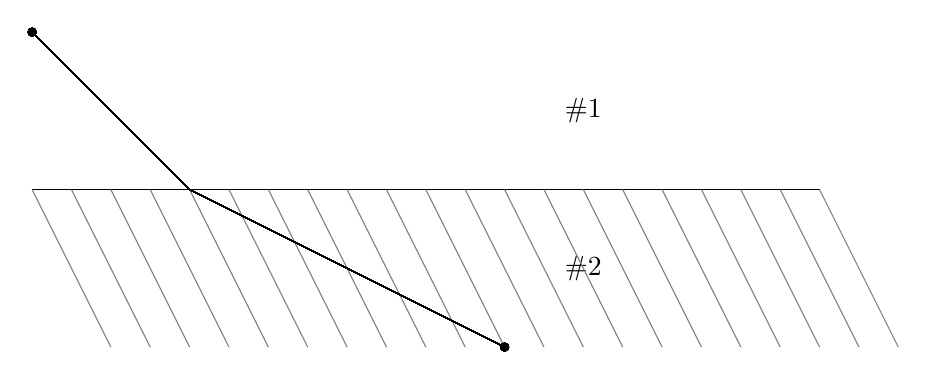
\begin{tikzpicture}
\node at (7, 1) {\#1};
\node at (7,-1) {\#2};
\draw (0,0)--(10,0);
\foreach \a in {0,...,20}{
\draw[color=black!50!white] (\a/2,0)--(\a/2+1,-2);
\draw (0,2)--(2,0)--(6,-2);
\draw[fill=black] (0,2) circle (0.05);
\draw[fill=black] (6,-2) circle (0.05);

}
\end{tikzpicture} \\ \\
This is the worst derivation ever.  Yet it reflects the equality of derivations we have in a typical Lagrangian mechanics textbook.  And likely, as must as Mr. Fermi had in mind.  \\ \\
We'll see his derivation wasn't much better, but at least he can get us to Schr\"{o}dinger.

\vfill

\begin{thebibliography}{}

\item Richard Feynman.  \textbf{Quantum Mechanics and Path Integrals} Dover, 2010.

\item Enrico Fermi.  \textbf{Quantum Mechanics} University of Chicago Press, 1961.

\end{thebibliography}

\end{document}